\appendix % Cue to tell LaTeX that the following "chapters" are Appendices

% Include the appendices of the thesis as separate files from the Appendices folder
% Uncomment the lines as you write the Appendices

% Appendix A

\chapter{Appendix} % Main appendix title
\label{AppendixA} % For referencing this appendix elsewhere, use \ref{AppendixA}

\section{Experimental Research from YNU}

\subsection*{Background of Research}
In recent years, laparoscopic surgery and robot-assisted surgery, which are less invasive than conventional open surgery, have become popular. Laparoscopic surgery is performed by making multiple 1 cm holes in the abdomen, inserting endoscopes and surgical forceps into the holes, and displaying the intra-abdominal conditions obtained through the endoscopes on a monitor. Laparoscopic surgery has a narrower field of view and provides less information than open surgery, making it difficult to master the technique. For this reason, surgical simulators for preoperative training have been developed to improve physicians' skills. The simulator is given the shape data and physical properties of organs obtained from CT scan data in advance. The position and posture of the surgical instruments are input by moving the instruments attached to the simulator, and the deformed state of the organs and the reaction force to the instruments are calculated as output. The reaction force is transmitted to the haptic device, the surgical tool, as a sensation, and the state of deformation is fed back to the surgeon by being projected on a monitor. In this study, we focus on the physical properties of organs to be input to the simulator. Current simulators use the physical properties of organs that have been processed, tested in vitro, and identified. However, the physical properties of organs in vivo differ from those of organs removed from the body due to cellular transformation and blood flow. Therefore, we believe that the physical property values obtained in in vitro tests may not reproduce the response of organs during surgery. Therefore, the purpose of this study is to identify the physical properties of the whole organ immediately after removal, which is closer to the in vivo state.

\subsection*{Physical Property Identification}
Various methods are used to identify physical properties. For example, there are methods that identify the Young's modulus from stress-strain curve obtained from a tensile test, and identify soft tissues by solving an inverse problem based on the results of strain measurement of the tissue using ultrasonic waves. As a method for identifying the physical properties of living organs, the viscoelastic properties of organs are identified by applying vibration to the organs to obtain material property data for use in surgical simulators, and by using the displacement captured by MRI. In this study, a nondestructive indentation test will be employed, which does not involve any treatment that alters the physical properties of the organ, such as damaging. At first, a load is applied to the organ, and the load applied to the organ and the deformation of the organ are measured. And simulate the model of the organ with the same geometry as in the experiment by applying a load to it. If the deformation is out of the acceptable range, the parameters given in the simulation are changed. Then, simulation is performed until the deformation is within the acceptable range, and the parameters obtained when the deformation is within the acceptable range are used as the physical properties of the organ immediately after removal.

\subsection*{Experimental Requirements}
The model is designed to identify the physical properties of organs by performing loading experiments on the organs and inverse analysis of the experimental results using CAE software. Since the internal tissues of organs are complex and the distribution of physical properties may not be uniform, the objective is to improve the accuracy of the model by loading at multiple locations and obtaining results for various deformation modes. Since the inverse analysis uses indentation and reaction forces as inputs, it is necessary to measure them simultaneously. In addition, since the accuracy is expected to be improved by considering the overall deformation as a constraint when determining material parameters in the inverse analysis, the overall deformation is also measured simultaneously. The purpose of this study is to construct a loading system that satisfies the above requirements and to measure the data for the inverse analysis.

\subsection*{Experimental Device}
The experimental apparatus is shown in Figure \ref{fig:expdeviceynu}.
A Workbee from Ooznest was used as the base actuator for the loading device. The loading device is controlled using G-code, which is used for NC machining. CNCShield for Arduino was used to issue commands to the loading device. In this study, the loading was applied vertically downward to the curved surface of the simulated organ (ellipsoid shape), so a small 6-axis force sensor manufactured by MinebeaMitsumi was used, which can measure reaction forces in directions other than the loading direction. The indentation depth was measured by the trigger voltage using G-code, and the trigger signal was recorded using National Instruments' USB-6003 and DAQ Express software. A spherical measuring element was attached to the tip of the loading rod to prevent breakage. The diameter of the measuring element was \SI{6}{\milli \meter}, and the material was ruby, which has a high level of both rigidity and sphericity. The simulated organs were made of Exseal's human skin gel (ultra-soft urethane resin) and molded into an ellipsoid shape. The deformation of the simulated organ was measured using KEYENCE's IX150 laser displacement meter and WAVE LOGGER X measurement software.

\begin{figure}%
	\centering
   \quad
   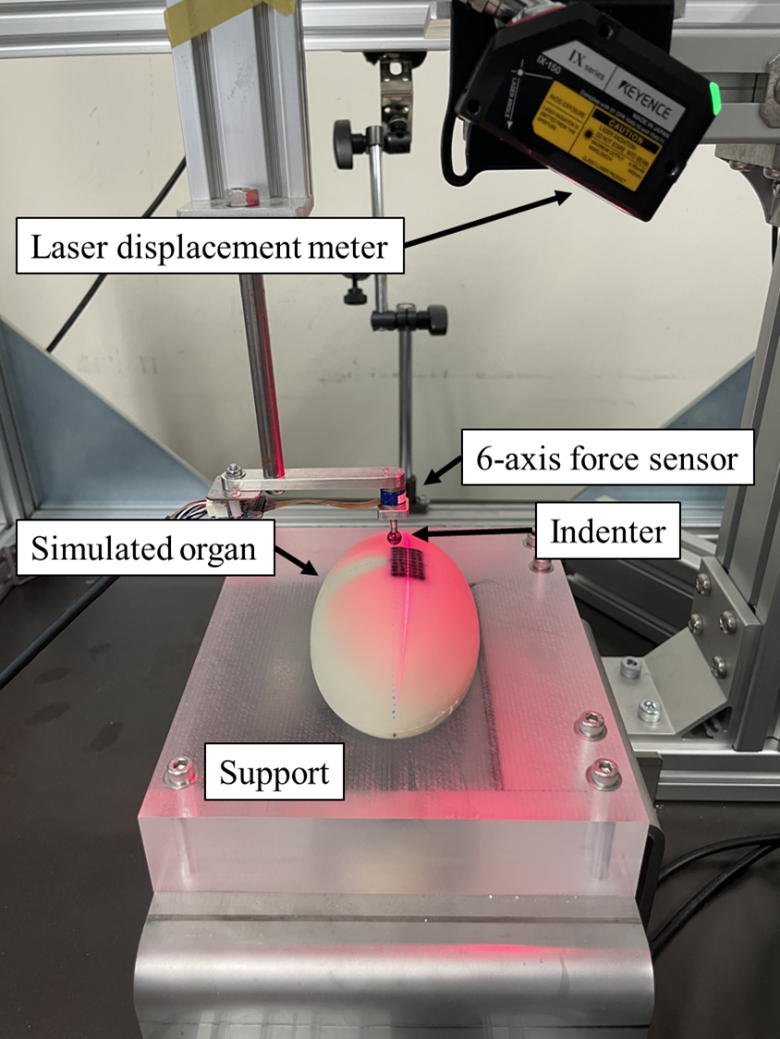
\includegraphics[width=10cm]{Images/appendix/ynu/fig1experimentaldevice.png}%
   \caption{Experimental device}%
   \label{fig:expdeviceynu}%
\end{figure}

\subsection*{Experimental Procedure}
The simulated organ to be loaded is shown in Figure \ref{fig:simorganynu} and a schematic diagram (top view) representing the coordinates of the loading points is shown in 
Figure \ref{fig:schemdiagynu}.
The loading points were set on the dotted line in Figure \ref{fig:schemdiagynu} because it was considered more suitable for parameter fitting if there were reaction forces of components other than the loading direction when performing the inverse analysis. The loading points were set at the top of the simulated organ and at a total of five points along the dotted line in
Figure \ref{fig:schemdiagynu}, moving with increments of $(\Delta X, \Delta Y) = (+2.5\,\mathrm{mm}, +2.5\,\mathrm{mm})$.\\
\begin{figure}%
	\centering
   \quad
   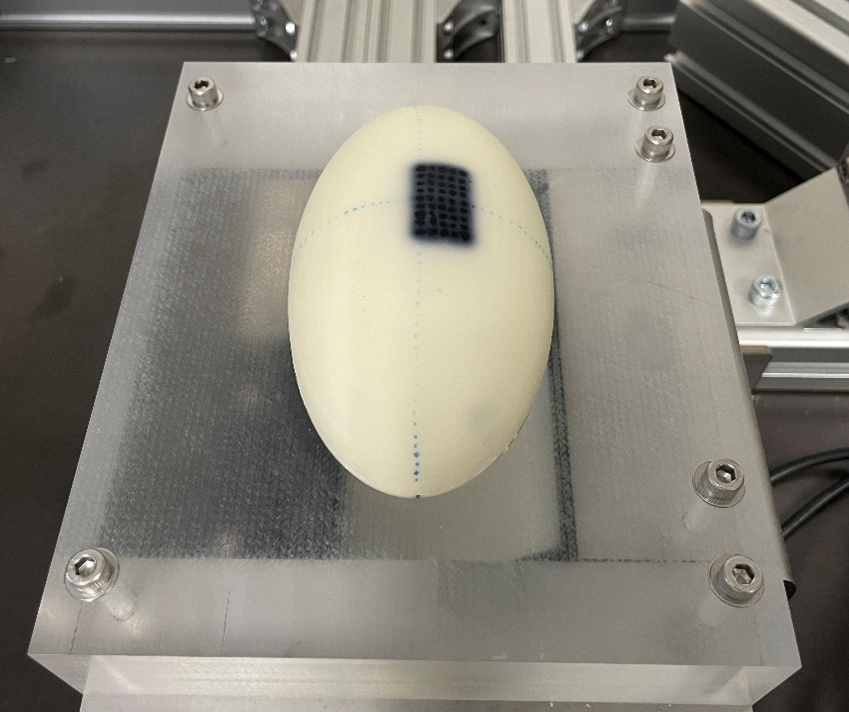
\includegraphics[width=10cm]{Images/appendix/ynu/fig2simulatedorgan.png}%
   \caption{Simulated organ}%
   \label{fig:simorganynu}%
\end{figure}
\begin{figure}%
	\centering
   \quad
   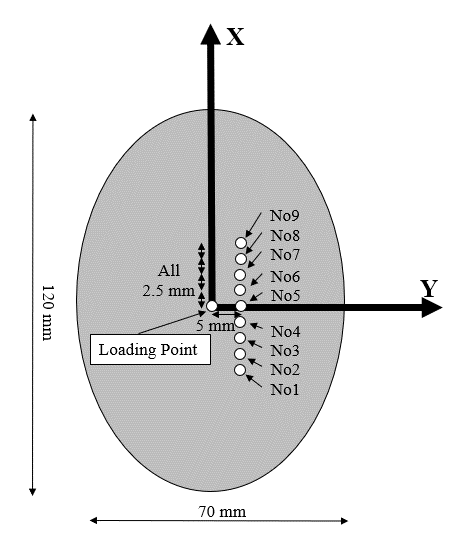
\includegraphics[width=8cm]{Images/appendix/ynu/fig3schematicdiagramrepresentingcoordinatesofloadingpoints_topview.png}%
   \caption[Schematic diagram YNU]{Schematic diagram representing coordinates of loading points (top view)}%
   \label{fig:schemdiagynu}%
\end{figure}

The experimental procedure is described below.
\begin{enumerate}
    \item Set the simulated organ on the table.
    \item Lubricate the loading point to eliminate the effect of friction.
    \item Move the measuring element directly above the loading point.
    \item Execute the G-code and start measuring the stroke, reaction force, and deformation.
    \item After the G-code is completed, terminate the measurement.
    \item Perform the same experiment 5 times for each loading point to confirm reproducibility.
\end{enumerate}

Experiments were conducted under room temperature environment (approx. \SI{20}{\degreeCelsius}).
The loading speed was \SI[per-mode = symbol]{30}{\milli \m\per \minute}, assuming the actual environment. 

\subsection*{Measurement method}
\subsubsection*{Measurement of indentation}
A $\SI{4}{\milli \m}$ load was applied to each loading point. The G code used in this study was designed to output a trigger voltage at a total of \SI{81}{}
times, and once when the bar was pushed in $\SI{0.1}{\milli \m}$.

These voltage changes were time-stamped using NI's USB-6003 and DAQ Express software. The indentation depth at the time of contact was set to
$\SI{0}{\milli \m}$, and the amount of indentation depth was measured as $\SI{0.1}{\milli \m}$ for each time the trigger voltage was transmitted. The sampling frequency was 
$\SI{10}{\kilo \hertz}$. An example of the voltage change during loading is shown in Figure \ref{fig:timevoltageynu}.\\
\begin{figure}%
	\centering
   \quad
   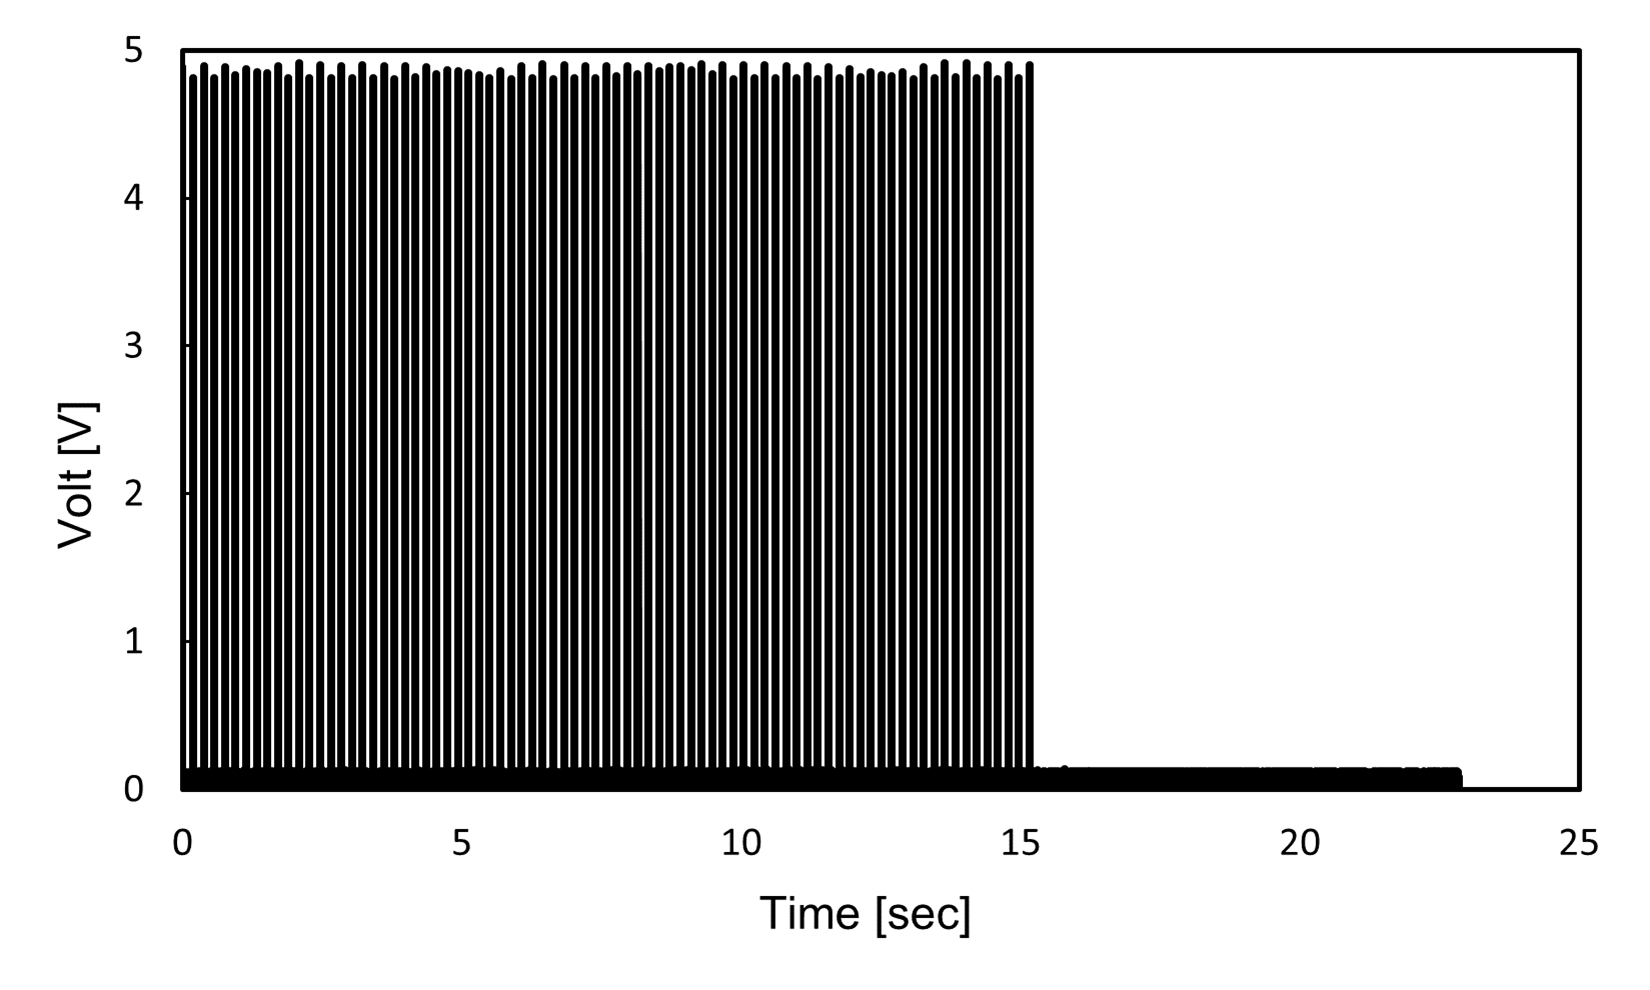
\includegraphics[width=10cm]{Images/appendix/ynu/fig4timehistoryoftriggervoltage.png}%
   \caption{Time history of trigger voltage}%
   \label{fig:timevoltageynu}%
\end{figure}
Because the reaction force and voltage were measured independently, the time axis was aligned by matching the peak time of the reaction force in the loading direction and the peak time of the push-in amount (Time when $\SI{4}{\milli \m}$ indented).

\subsubsection*{Measurement of reaction forces}
The specifications of the compact 6-axis force sensors are shown in Figure \ref{fig:specsensorynu}. 
\begin{figure}%
	\centering
   \quad
   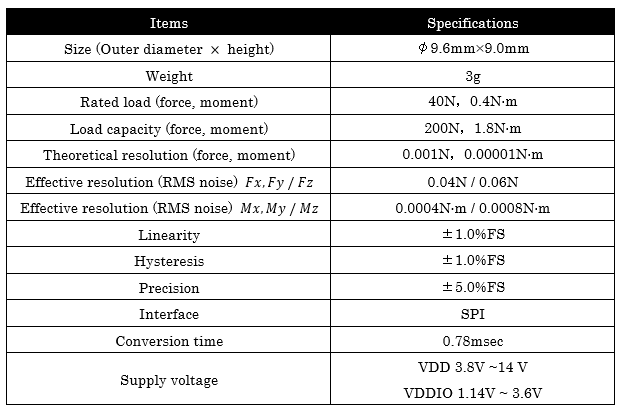
\includegraphics[width=10cm]{Images/appendix/ynu/tab1specificationsofminiature6axisforcesensors.png}%
   \caption{Specifications of miniature 6-axis force sensors}%
   \label{fig:specsensorynu}%
\end{figure}
The sampling frequency was $\SI{1000}{\hertz}$. To reduce the effect of initial drift, we waited five minutes to stabilize after sensor startup.

\subsubsection*{Measurement of deformation}
Figure \ref{fig:defmeasureynu} shows the laser beam on a straight line. Since the laser displacement meter was run with the same trigger voltage as the stroke measurement, the time when the deformation was measured was based on the time axis of the stroke.
\begin{figure}%
	\centering
   \quad
   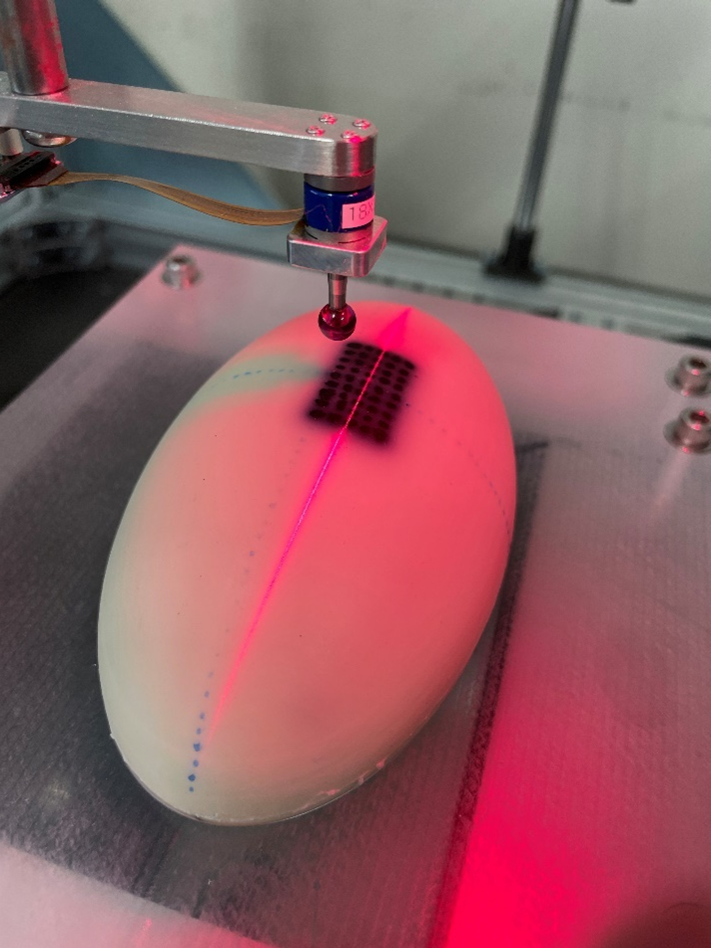
\includegraphics[width=8cm]{Images/appendix/ynu/fig5laserlineonthesimulatedorgan.png}%
   \caption{Deformation measurement}%
   \label{fig:defmeasureynu}%
\end{figure}

\subsection*{Experimental results}
The time history of the reaction force in the loading direction when the top of the simulated organ is loaded is shown 
in Figure \ref{fig:forcemeasurementynu}, and the deformation is shown in Figure \ref{fig:defmeasurementynu}. 
We performed five loading experiments to ensure reproducibility. The measurement accuracy of the laser displacement meter is
$\SI{0.05}{\milli \m}$.

The experimental results show that the deformation of the simulated organ at symmetrically located points, such as measurement points No. \SI{4}{} and No. \SI{6}{} (Fig. \ref{fig:disstroke}), are in good agreement with the results obtained by the laser displacement meter. The results indicate the possibility of using the deformation state obtained by laser displacement meter for the identification of physical properties in the future.
\begin{figure}
    \centering
    \begin{subfigure}[b]{0.45\textwidth}
    \centering
    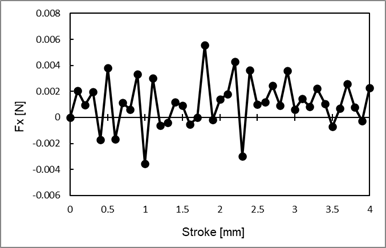
\includegraphics[width=\textwidth]{Images/appendix/ynu/fig6forcestroke_a.png}
    \caption{Force component in x-direction}
    \label{fig:forcezxnu}
    \end{subfigure}
    \hfill
    \begin{subfigure}[b]{0.45\textwidth}
    \centering
    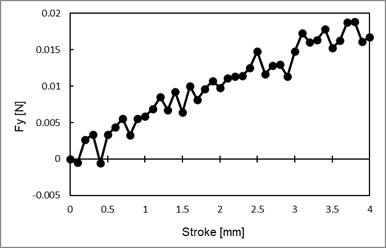
\includegraphics[width=\textwidth]{Images/appendix/ynu/fig6forcestroke_b.png}
    \caption{Force component in y-direction}
    \label{fig:forceyynu}
    \end{subfigure}
    \vspace{0.5cm}
    \begin{subfigure}[b]{0.45\textwidth}
    \centering
    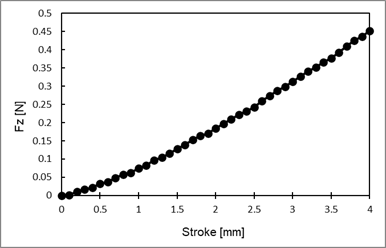
\includegraphics[width=\textwidth]{Images/appendix/ynu/fig6forcestroke_c.png}
    \caption{Force component in z-direction}
    \label{fig:forcezynu}
    \end{subfigure}  
    \hspace{0.3cm}
    \caption{Reaction force components results}
    \label{fig:forcemeasurementynu}
\end{figure}

\begin{figure}
    \centering
    \begin{subfigure}[b]{0.5\textwidth}
    \centering
    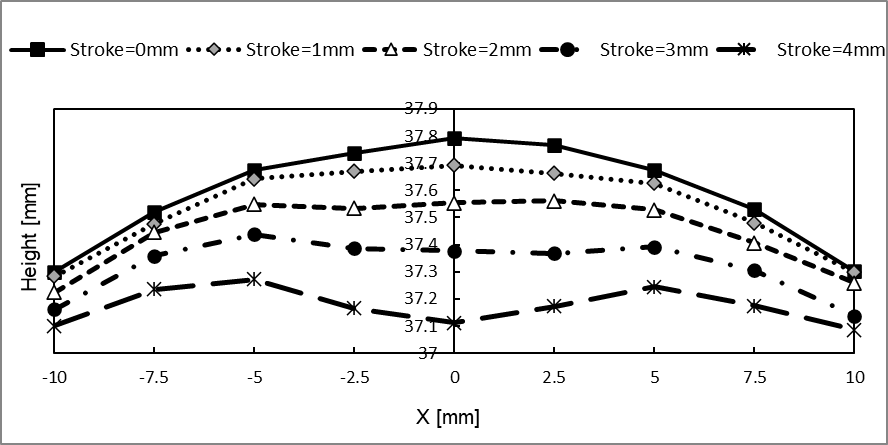
\includegraphics[width=\textwidth]{Images/appendix/ynu/fig7hightprofiletransition.png}
    \caption{Height profile transition}
    \label{fig:heighttrans}
    \end{subfigure}
    \hfill
    \begin{subfigure}[b]{0.5\textwidth}
    \centering
    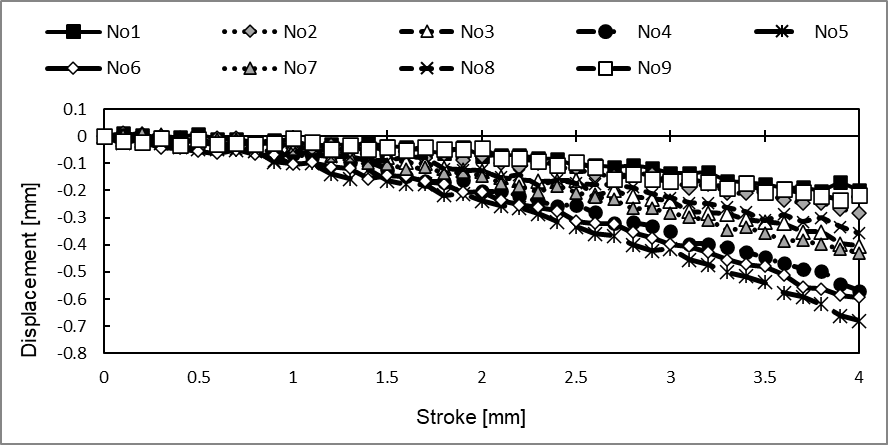
\includegraphics[width=\textwidth]{Images/appendix/ynu/fig8displacementsstroke.png}
    \caption{Displacement stroke}
    \label{fig:disstroke}
    \end{subfigure}
    \vspace{0.5cm}
    \caption{Deformation results}
    \label{fig:defmeasurementynu}
\end{figure}

%-----------------------------------------------------
\section{MATLAB Code}
\subsection*{NRMSE Polynomial Second Degree}

\lstset{style=matlab} % set the style to MATLAB
\begin{lstlisting}
   %Variables
   Mu = ...
   [0.0085415 0.012453 0.0099752 0.0099604 0.0099896 0.012315 0.0099752 0.0078715 0.0078906 0.007927 0.006500 0.006819 0.007153 0.007872 0.008258 0.008662 0.009087 0.009533 0.01 0.0099988 0.0099991 0.0099997 0.015 0.012 0.012 0.010867 0.010894 0.01092 0.0122 0.0132 0.0142 0.0122 0.0115 0.0142 0.0099 0.0098 0.0097 0.0101];
  
  D_1 = ...
   [5.25 139.31 127.51 127.8 128.6 131.62 5.25 1.0085 1.0085 4.1115 1 1 5 5 10 10 80 80 160 5.8429 5.8262 5.7867 50 50 1 47.199 48.454 49.677 72.8369 1.0017 1 159.683 1.002 101.3 50 50 50 50];
  
  NRMSE = ...
   [0.175 0.065 0.226 0.228 0.229 0.064 0.034 0.249 0.248 0.248 0.437 0.381 0.343 0.255 0.218 0.169 0.235 0.193 0.268 0.0339 0.0342 0.0339 0.4106 0.1197 0.2659 0.0343 0.0351 0.0352 0.08339 0.41757 0.539562 0.09984 0.20519 0.17806 0.103 0.114 0.124 0.0844];
  
  X = transpose([Mu; D_1]);
  y = NRMSE;
  
  %Polynomial degree 2
         p00 =       2.798;
         p10 =        -535;
         p01 =    0.009251;
         p20 =   2.654e+04;
         p11 =      -1.022;
         p02 =   1.467e-05;
  f = @(x) (p00 + p10*x(1) + p01*x(2) + p20*x(1)^2 + p11*x(1)*x(2) + p02*x(2)^2);
  
  %Setting the upper and lower boundaries
  lb = [0.0001, 1];
  ub = [1, 1000];

  %Finding the minimum
  [xmin,FVAL] = fmincon(f, [0.012453, 139.31], [], [], [], [], lb, ub);
\end{lstlisting}

\subsection*{MRE Polynomial Fourth Degree}

\lstset{style=matlab} % set the style to MATLAB

\begin{lstlisting}
%Variables
Mu = ...
 [0.0085415 0.012453 0.0099752 0.0099604 0.0099896 0.012315 0.0099752 0.0078715 0.0078906 0.007927 0.0065 0.006819 0.007153 0.007872 0.008258 0.008662 0.009087 0.009533 0.01 0.0099988 0.0099991 0.0099997 0.015 0.012 0.012 0.010867 0.010894 0.01092 0.0122 0.0132 0.0142 0.0122 0.0115 0.0142 0.0099 0.0098 0.0097 0.0101 0.0122 0.0119 0.0101 0.0099 0.0105];

D_1 = ...
 [5.25 139.31 127.51 127.8 128.6 131.62 5.25 1.0085 1.0085 4.1115 1 1 5 5 10 10 80 80 160 5.8429 5.8262 5.7867 50 50 1 47.199 48.454 49.677 72.8369 1.0017 1 153.68 1.002 101.3 50 50 50 50 108.66 72.7 5.5 5.5 5.5];

MRE = ...
 [0.2188 0.1713 0.2916 0.2928 0.2929 0.1697 0.1098 0.273 0.2715 0.2726 0.4153 0.3706 0.3444 0.2786 0.253 0.2175 0.288 0.2588 0.3241 0.1103 0.1104 0.1098 0.2831 0.1479 0.2183 0.1207 0.1219 0.1218 0.1388 0.3086 0.386 0.2012 0.1847 0.1717 0.1838 0.1914 0.1983 0.1689 0.1429 0.1331 0.1111 0.1105 0.125];

X = transpose([Mu; D_1]);
y = MRE;

%Polynomial degree 4
p00 =      -6.509;
p10 =        3317;
p01 =    -0.07093;
p20 =  -5.609e+05;
p11 =       23.91;
p02 =  -0.0003905;
p30 =   3.927e+07;
p21 =       -2470;
p12 =     0.07195;
p03 =  -2.663e-07;
p40 =  -9.728e+08;
p31 =   7.912e+04;
p22 =      -3.035;
p13 =   8.145e-06; 
p04 =    4.08e-10;

f =  @(x) (p00 + p10*x(1) + p01*x(2) + p20*x(1)^2 + p11*x(1)*x(2) + p02*x(2)^2 + p30*x(1)^3 + p21*x(1)^2*x(2) + p12*x(1)*x(2)^2 + p03*x(2)^3 + p40*x(1)^4 + p31*x(1)^3*x(2) + p22*x(1)^2*x(2)^2 + p13*x(1)*x(2)^3 + p04*x(2)^4);

%Setting the upper and lower boundaries
lb = [0.007, 0.1];
ub = [0.013, 100];

%Finding the minimum
[xmin,FVAL] = fmincon(f, [0.012453, 139.31], [], [], [], [], lb, ub);

x = linspace(0.0001, 0.1, 20);
y = linspace(5,1000, 20);
\end{lstlisting}